%% TAS 2026 (AAAI Fall Symposium Series), CAMERA-READY VERSION.
%% Single author, de-anonymised. Addresses all reviews of submission 7658.
%%
%% Formatted with the official AAAI-27 author kit (aaai2027.sty/.bst, template
%% version 2027.1), as the AAAI Press proceedings instructions require.
%% The style requires pdfLaTeX; it stops under XeLaTeX or LuaLaTeX.
%%
%% Build: pdflatex -> bibtex -> pdflatex -> pdflatex
%% External files: figures/fig1_censoring_bias.pdf, figures/fig2_horizon_survival.pdf
%% Every number is regenerated by scripts/censoring/reproduce_all.py and
%% scripts/censoring/revision_analysis.py.

\documentclass[letterpaper]{article} % DO NOT CHANGE THIS
\usepackage{aaai2027}  % DO NOT CHANGE THIS
% Fonts (newtxtext, helvet, courier) are loaded by aaai2027.sty.
\usepackage[hyphens]{url}  % DO NOT CHANGE THIS
\usepackage{graphicx} % DO NOT CHANGE THIS
\urlstyle{rm} % DO NOT CHANGE THIS
\def\UrlFont{\rm}  % DO NOT CHANGE THIS
\usepackage{natbib}  % DO NOT CHANGE THIS AND DO NOT ADD ANY OPTIONS TO IT
\usepackage{caption} % DO NOT CHANGE THIS AND DO NOT ADD ANY OPTIONS TO IT
\frenchspacing  % DO NOT CHANGE THIS

\usepackage{booktabs}
\usepackage{amsmath}
\usepackage{amssymb}

\pdfinfo{
/TemplateVersion (2027.1)
}

\setcounter{secnumdepth}{2}

\newcommand{\pb}{\bar\pi}
\newcommand{\rev}{$^{\dagger}$}

\title{Invalid Is Not Failure:\\
Infrastructure Censoring Bias in Long-Horizon Agent Evaluation}

\author{
    Shilin Chhabra
}
\affiliations{
    University of Wisconsin--Madison\\
    chhabra7@wisc.edu
}

\begin{document}
\maketitle

\begin{abstract}
Long-running agents sometimes stop without a valid task outcome because a
provider, runtime, or harness failed rather than the agent. Benchmarks then
score such runs as failures or drop them. We treat this as an identification
problem. When infrastructure failures are independent of the agent, each common
policy is a closed-form function of three numbers: the success rate and the
mean survival probabilities of successful and failed runs. Scoring invalid runs
as failures multiplies the success \emph{probability} by the survival of
successes, so it never overstates reliability yet can reverse model
comparisons. Dropping them multiplies the success \emph{odds} by the survival
ratio, so it overstates reliability when successes survive better and
understates it otherwise. Rerunning removes only the between-task part of that
distortion. A Kaplan--Meier-weighted estimator that uses only observed failure
times recovers reliability, including under step-dependent hazards. Applying
hypothetical per-step hazards to 80{,}036 SWE-agent and 4{,}950 $\tau$-bench
trajectories exposes very different sensitivities: at a 1\% hazard, dropping
shifts reliability by $+1.5$ and $+0.2$ points, scoring as failure by $-2.3$ and
$-6.8$, and a 0.32\% hazard already reverses a $\tau$-bench model pair. The
SWE-agent corpus also contains 3{,}176 runs ended by container runtime errors
and scored as task failures, which leave its reliability identified only within
$[16.7\%, 20.7\%]$. We give a rule for separating censoring from failure and a
minimum validity record for benchmark reports.
\end{abstract}

\section{Introduction}

A long-horizon agent run can end for two very different reasons. The agent can
fail the task, or the measurement apparatus can fail the agent: a provider quota
is exhausted, an API returns 503, a container dies, a harness process crashes.
Only the first is evidence about the agent. Yet benchmark reports usually
collapse both into one success rate through an unstated policy: invalid runs are
either scored as failures or deleted.

Validity problems in agent benchmarks are well documented
\citep{kapoor2024agentsthatmatter,weidinger2025evalscience,zhu2026guardrails},
and a recent audit finds that agent benchmark papers disclose little about their
harness and failure handling \citep{moghadasi2026disclose}. Our question is
narrower: what does each handling policy estimate? The answer is structural.
Suppose infrastructure failures are entirely independent of the agent, arriving
with a small constant hazard $q$ per agent step. A run of horizon $H$ then
survives with probability $s^{H}$, $s=1-q$. Long runs are exposed more often,
so an outcome-\emph{independent} per-step failure becomes informative \emph{at
the trajectory level} whenever horizon and success are associated.

We use \emph{censoring} operationally: termination before a semantic endpoint is
observed, which induces missing binary outcomes. We keep three run states
distinct: a valid success, a valid failure, and an infrastructure-invalid
(censored) run whose outcome was never observed.

\vspace{2pt}
\noindent\textbf{Contributions.}
\begin{itemize}\itemsep1pt \parskip0pt \topsep2pt
\item \textbf{Formal.} A validity rule; assumption-free bounds; a three-number
characterisation of the invalid-as-failure and drop policies; a rerun
decomposition; and a weighting estimator that needs only observed quantities
(Section~\ref{sec:model}).
\item \textbf{Empirical.} On two public corpora ($\approx$85k trajectories), the
size of each distortion under declared hazards, the hazards at which rankings
break, and an observed case of container failures already scored as task
failures (Sections~\ref{sec:setup}--\ref{sec:results}).
\item \textbf{Practice.} A minimum validity record for benchmark reports
(Section~\ref{sec:practice}).
\end{itemize}

\section{Identification Under Censoring}
\label{sec:model}

\paragraph{Estimand.} A benchmark initiates runs $i=1,\dots,N$ with fixed
semantic outcomes $Y_i\in\{0,1\}$ and horizons $H_i$ (agent decision steps). The
estimand is the corpus reliability $p=N^{-1}\sum_i Y_i$. Randomness enters only
through the validity indicators $C_i$ (1 if $Y_i$ is observed), drawn by the
infrastructure with $\pi_i=\Pr(C_i=1)$. This design-based view matches the
finite corpora we analyse; population statements would additionally need
i.i.d.\ sampling of runs, which we do not assume.

\paragraph{Definition 1 (Validity rule).} Fix the benchmark specification, which
declares the agent's budgets (steps, tokens, cost, context window, wall-clock)
and environment. An interruption at step $k$ is an \emph{outcome} (a valid
failure) if a fault-free execution with the same agent actions up to $k$ would
also have terminated there: budget or context exhaustion, or damage the agent
did to its own environment. It is \emph{censoring} if the fault-free execution
would not have terminated: provider errors and quotas, host preemption, harness
defects, and wall-clock timeouts whose budget was consumed by infrastructure
latency or retries. Interruptions that cannot be attributed either way are a
third, reported category and are handled by bounds. The context window is part
of the system under test, so context exhaustion is a valid failure and $p$ is
success within the declared budgets. Budgets are best declared in
agent-controlled units (steps, tokens) so the rule is decidable from logs.

\paragraph{Proposition 1 (Assumption-free bounds).}
Let $M$ be the censored count and $S$ the observed successes. With no
assumption about the outcomes of censored runs,
\begin{equation}
S/N \;\le\; p \;\le\; (S+M)/N .
\label{eq:bounds}
\end{equation}
\emph{Proof.} Each censored run has an unknown $Y_i\in\{0,1\}$; setting all to
$0$ or all to $1$ gives the endpoints.\hfill$\square$

This is the agent-evaluation instance of a classical worst-case bound
\citep{manski1990nonparametric}. It reframes invalid-as-failure, $S/N$, as the
\emph{lower endpoint of the identified interval} rather than an estimate. For
bounded scores $Y_i\in[a,b]$ (partial credit, judge scores) the endpoints become
$(\sum_i C_iY_i+aM)/N$ and $(\sum_i C_iY_i+bM)/N$, and everything below holds
unchanged; for unbounded metrics such as cost the bounds are infinite and any
report rests on assumptions.

\paragraph{Observation model.} Let $T_i$ be the step at which infrastructure
would first fail run $i$, independent of $(Y_i,H_i)$, with survival
$G(h)=\Pr(T>h)$. Run $i$ is valid iff $T_i>H_i$, so $\pi_i=G(H_i)$. The
constant-hazard case is
\begin{equation}
\pi_i = s^{H_i},\qquad s=1-q .
\label{eq:pi}
\end{equation}
Write $\pb_1$ and $\pb_0$ for the mean of $\pi_i$ over successful and failed
runs, $\pb=p\pb_1+(1-p)\pb_0$ for the overall mean (so $m=1-\pb$ is the
expected invalid fraction), and $\rho=\pb_1/\pb_0$ for the \emph{survival
ratio}.

\paragraph{Proposition 2 (Three numbers determine both policies).}
For any observation probabilities $\pi_i$, even outcome-dependent ones (the
model above only determines their values),
\begin{align}
\mathbb{E}[\hat p_{\mathrm{fail}}] &= p\,\pb_1 \;\le\; p, \label{eq:fail}\\
\frac{p_{\mathrm{cc}}}{1-p_{\mathrm{cc}}} &= \rho\,\frac{p}{1-p},
\quad\text{i.e.}\quad
p_{\mathrm{cc}}-p=\frac{p(1-p)(\pb_1-\pb_0)}{\pb}, \label{eq:cc}
\end{align}
where $\hat p_{\mathrm{fail}}=N^{-1}\sum_iC_iY_i$ and $p_{\mathrm{cc}}=\sum_i
\pi_iY_i/\sum_i\pi_i$ is the complete-case induced estimand (the probability
limit of $S/(N-M)$, not its exact finite-sample mean). In expectation
\eqref{eq:bounds} is $[p\pb_1,\;p\pb_1+m]$.
\emph{Proof.} $\sum_i\pi_iY_i=Np\pb_1$, $\sum_i\pi_i(1-Y_i)=N(1-p)\pb_0$, and
$\hat p_{\mathrm{fail}}$ is linear in $C$.\hfill$\square$

Scoring as failure multiplies the success \emph{probability} by $\pb_1$; dropping
multiplies the success \emph{odds} by $\rho$. Three consequences follow.
\emph{(i) Direction.} Invalid-as-failure never overstates $p$. Complete-case
overstates $p$ iff $\rho>1$ (successes survive better) and understates it iff
$\rho<1$, in which case \emph{both} policies err downward. The two policies err
in opposite directions only when $\rho>1$.
\emph{(ii) Conservatism.} Invalid-as-failure is conservative for one agent's
level but not for comparisons: the gap $p_A\pb_{1A}-p_B\pb_{1B}$ can shrink,
grow, or change sign relative to $p_A-p_B$, because each agent is discounted by
its own survival of successes.
\emph{(iii) Horizon distribution, not mean.} Under \eqref{eq:pi},
$\pb_y(s)=\mathbb{E}[s^H\mid Y=y]$ is the probability generating function of
the horizon of outcome $y$, so $\rho$ depends on the whole outcome-conditional
horizon distributions. The mean gap enters only to first order,
$\log\rho=q(\bar H_0-\bar H_1)+O(q^2)$. First-order stochastic dominance of
failure horizons over success horizons is sufficient for $\rho>1$ at every $q$
but not necessary.

\paragraph{Proposition 3 (Rerun until valid).}
Group runs into cells $c$ (task $\times$ agent) with within-cell law $F_c$ and
weight $w_c$. If each invalid attempt is replaced by an independent fresh
attempt from $F_c$ until one is valid, the accepted attempt has law
proportional to $G(H)\,dF_c$, and
\begin{align}
p_{\mathrm{rerun}}-p&=\textstyle\sum_c w_c\,
\mathrm{Cov}_c(Y,\pi)/\mathbb{E}_c[\pi],\label{eq:rerun}\\
p_{\mathrm{cc}}-p&=\big[\textstyle\sum_c w_c\mathrm{Cov}_c(Y,\pi)
+\mathrm{Cov}_w(p_c,\mathbb{E}_c[\pi])\big]/\pb .\nonumber
\end{align}
Rerunning removes the between-cell (composition) term but keeps a within-cell
tilt towards attempts that happened to be short. It is exact for deterministic
agents ($\mathrm{Cov}_c=0$) and costs $\sum_cw_c/\mathbb{E}_c[\pi]$ attempts per
task in expectation. \emph{Proof.} Appendix~A.1.

\paragraph{Proposition 4 (Weighting from observables).}
If the true $\pi_i>0$ are known, the Horvitz--Thompson estimator $\hat
p_{\mathrm{HT}}=N^{-1}\sum_iC_iY_i/\pi_i$ is exactly unbiased for $p$, since
$\mathbb{E}[C_i/\pi_i]=1$
\citep{horvitz1952generalization,robins1994estimation}. In deployment $\pi$ is
unknown but \emph{no counterfactual horizon is needed}: only valid runs are
weighted, and their $H_i$ is observed. Each run reveals $V_i=\min(H_i,T_i)$ and
$C_i$, so $G$ is estimable by Kaplan--Meier with infrastructure failure as the
event and completion as censoring
\citep{kaplan1958nonparametric,robins2000correcting,satten2001kaplan}. The
H\'ajek estimator
\begin{equation}
\hat p_{\mathrm{KM}}=\textstyle\sum_iC_iY_i/\hat G(H_i)\,\big/\,\sum_iC_i/\hat G(H_i)
\label{eq:km}
\end{equation}
is consistent under $T\perp(Y,H)$ (optionally within strata such as provider)
and positivity, $G>0$ on the support of $H$. Under \eqref{eq:pi} the hazard
MLE is $\hat q=M/\sum_iV_i$. Weighting cannot repair positivity failures such as
a hard quota, nor outcome-dependent censoring.

\paragraph{Three levels of reporting.} \emph{(L1) No assumptions:} report
\eqref{eq:bounds}. \emph{(L2) Non-informative observation} ($\rho=1$): the
complete-case rate is justified. \emph{(L3) Independent infrastructure
failure:} report \eqref{eq:km}, with its assumption stated.

\section{Setup}
\label{sec:setup}

\paragraph{Corpora.} \emph{Primary:} 80{,}036 SWE-agent
\citep{yang2024sweagent} trajectories \citep{nebius2024trajectories}
(CC-BY-4.0) on SWE-bench-style tasks
\citep{jimenez2024swebench,openai2024swebenchverified}, each with a
ground-truth resolution label from test execution; we read five pruned columns.
\emph{Secondary:} 4{,}950 $\tau$-bench trajectories
\citep{agentsuite2026taubench,yao2025taubench} from 30 per-model files (29
distinct model identifiers), 165 tasks per file, strictly binary score. We keep
every labelled row, including one SWE row with $H=0$ ($\pi=1$). By
Definition~1, eight of SWE-agent's nine exit statuses are outcomes (submission,
context or cost exhaustion, malformed output; Appendix~A.7); the ninth,
\texttt{early\_exit}, is unattributable (Section~\ref{sec:results}).

\paragraph{Horizon.} $H$ counts agent decision turns only, excluding system,
user, and tool turns. The definition was fixed before any censoring result, and
an independent recount of 20 re-fetched trajectories per corpus agreed exactly
(20/20 in both).

\paragraph{Censoring is semi-synthetic.} We inject censoring into completed,
labelled corpora. The per-step hazard grid, $q\in\{0, 0.1, 0.25, 0.5, 1,
2\}\%$, was predeclared and is a \textbf{sensitivity analysis, not a measured
outage rate};
because the identities are exact under the injected mechanism, agreement between
simulation and theory checks the code, not the model. The empirical content is
the outcome-horizon structure of real trajectories, which fixes how much a given
hazard would distort each policy. Monte Carlo intervals (200 replicates) reflect injected
censoring only. Analyses marked \rev{} were added after review, use a separate
seed, and leave every predeclared quantity unchanged.

\section{Results}
\label{sec:results}

\begin{table}[t]
\centering
\small
\setlength{\tabcolsep}{3.6pt}
\begin{tabular}{@{}lrrrrrrr@{}}
\toprule
corpus & $p$ & $\pb_1$ & $\pb_0$ & $\rho$ & $m$ & drop & fail \\
\midrule
SWE-agent & 16.73 & .864 & .777 & 1.113 & 20.9 & $+1.54$ & $-2.27$ \\
$\tau$-bench & 55.03 & .877 & .869 & 1.009 & 12.6 & $+0.23$ & $-6.75$ \\
\bottomrule
\end{tabular}
\caption{Cross-domain summary at a hypothetical $q=1\%$: mean survival of
successes and failures, survival ratio $\rho$, invalid fraction $m$ (\%), and
policy biases (points). By \eqref{eq:fail}--\eqref{eq:cc} these three numbers
reproduce both biases exactly (error $<10^{-15}$).}
\label{tab:cross}
\end{table}

\begin{figure*}[t]
\centering
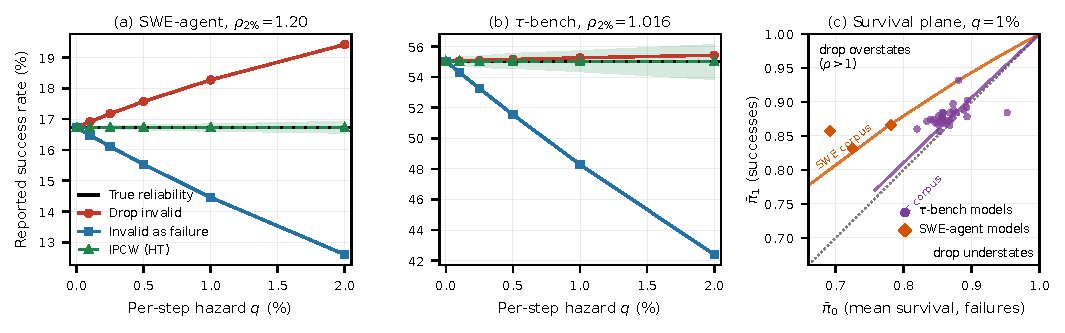
\includegraphics[width=\textwidth]{figures/fig1_censoring_bias.pdf}
\caption{\textbf{Synthetic sensitivity analysis}: $q$ is a declared parameter,
not a measured outage rate. \textbf{(a, b)} Reported reliability against $q$.
SWE-agent successes survive much better ($\rho=1.20$ at $q=2\%$), so dropping
invalid runs inflates reliability; on $\tau$-bench $\rho\approx1$, so the
complete-case curve is almost flat while invalid-as-failure falls sharply. IPCW
tracks the truth (shaded: 95\% Monte Carlo interval, 200 replicates). Note the
different $y$ ranges. \textbf{(c)}\rev{} Survival plane: lines trace each
corpus from $q=0$ (top right) to $q=2\%$; points are models at $q=1\%$. Above
the diagonal dropping overstates reliability; 5 of 29 $\tau$-bench models lie
below it.}
\label{fig:main}
\end{figure*}

\paragraph{Three numbers explain the dissociation.} On SWE-agent the survival
ratio is well above one ($\rho=1.11$ at $q=1\%$, $1.20$ at $2\%$), so
complete-case reporting inflates reliability ($+1.54$ and $+2.69$ points) while
invalid-as-failure deflates it ($-2.27$ and $-4.12$): a 6.8-point spread between
two defensible policies on identical data at $q=2\%$. On $\tau$-bench
$\rho=1.009$, so the complete-case bias nearly vanishes ($+0.40$ at $2\%$), but
invalid-as-failure is \emph{worse} ($-12.64$) because it scales with the base
rate: $p(1-\pb_1)$ with $p=55\%$ (Table~\ref{tab:cross},
Figure~\ref{fig:main}).

\paragraph{The mean gap is not enough.\rev} The first-order approximation
$\log\rho\approx q(\bar H_0-\bar H_1)$ overstates SWE-agent's $\log\rho$ by 26\%
at $q=1\%$ (0.135 vs.\ 0.107) and 48\% at $2\%$: $s^H$ is convex in $H$, so
the long tail of failed runs lowers $\pb_0$ less than their mean suggests. Neither corpus satisfies stochastic
dominance: the outcome-conditional horizon distributions cross at short
horizons ($h=3$ for SWE-agent, $h=8$ for $\tau$-bench; Figure~\ref{fig:horizon}), yet $\rho>1$ at every
$q\le5\%$ in both. The sign is therefore an empirical property to be checked,
not a consequence of the mean gap.

\paragraph{Both policies can err downward.\rev} At model level, 5 of 29
$\tau$-bench models have $\rho<1$ (Figure~\ref{fig:main}c): their successes are
longer, so complete-case reporting also understates reliability. For
Qwen3-235B-A22B-Instruct-2507 at $q=1\%$ the two policies give $-1.78$ and $-4.71$
points. Across models the complete-case bias ranges from $-1.78$ to $+1.01$
points and the invalid-as-failure bias from $-9.83$ to $-0.91$.

\paragraph{Comparisons break at small hazards.\rev} Solving the closed forms on
a fine grid, the first $\tau$-bench pairwise reversal (29 models, 406 pairs)
occurs at $q=0.32\%$ under invalid-as-failure and $0.44\%$ under complete-case,
when only 4.3\% and 5.8\% of runs are invalid; the median gap between adjacent
models is 1.2 points. At $q=2\%$ invalid-as-failure reverses 11 pairs and
complete-case 2 (Kendall $\tau_b=0.939$ and $0.984$). Invalid-as-failure moves the $\tau$-bench
level by a full point at $q=0.14\%$ ($m=1.9\%$). SWE-agent's 3 eligible models
show no reversal at any predeclared hazard, a weak test we report as such.

\paragraph{Rerunning removes most, not all, of the bias.\rev} SWE-agent has
4{,}219 task$\times$model cells (median 13 runs each). By \eqref{eq:rerun},
rerunning until valid removes 70--72\% of the complete-case bias at every hazard,
leaving $+0.44$ points at $q=1\%$ and $+0.75$ at $2\%$ from the within-cell
tilt, at a cost of 1.28 and 1.60 attempts per task. On $\tau$-bench 93\% of
cells hold a single trajectory, so the within-cell term is not identified.

\paragraph{Weighting works from observables.\rev} Simulating failure times step
by step and estimating $G$ only from $(V_i,C_i)$, the Kaplan--Meier H\'ajek
estimator \eqref{eq:km} has bias at most $0.015$ points (SWE-agent) and
$0.008$ ($\tau$-bench) under constant hazards up to 2\%. Under a hazard that
doubles after step 25 it stays within $0.024$ points, whereas a
constant-hazard fit is biased by $+0.33$ and $+0.67$ points at base hazards of
$0.5\%$ and $1\%$ (SWE-agent; Appendix~A.6). Estimated weights are even
\emph{more} efficient than true ones (standard deviation 0.25 vs.\ 0.37 points
on $\tau$-bench at $q=1\%$), as expected \citep{robins1994estimation}. A hard
cap behaves differently: if every run beyond 25 steps is invalidated, $T$ is
still independent of $(Y,H)$ but $G=0$ past the cap, so the weights collapse to
the complete case (23.04\% vs.\ true 16.73\% on SWE-agent) and only
\eqref{eq:bounds}, $[15.05, 49.73]\%$, remains valid.

\paragraph{Bounds are wide.} At $q=1\%$ the expected identified intervals are
$[14.5,35.3]$ (SWE-agent) and $[48.3,60.9]$ ($\tau$-bench): a single number
without a stated mechanism is a strong assumption.

\paragraph{Observed container failures.\rev} The SWE-agent corpus already
contains real invalidation. Its \texttt{early\_exit} status is set only when the
container runtime raises during a step (a failed command, a broken pipe, or an
interrupt that fails after a timeout), followed by a container reset
\citep{sweagent2024code}. It marks 3{,}176 runs (4.0\%), none resolved, all
scored as task failures in the corpus labels. Under Definition~1 these are
unattributable: a failed interrupt may follow an agent command that hung. The
implied constant hazard is $\hat q=0.15\%$ per step, inside our grid, and
per-band estimates (0.11--0.22\%) are roughly flat in step. The three reporting
levels give: L1 $[16.73,20.70]\%$; complete-case $17.42\%$; L3
model-stratified \eqref{eq:km} $17.09\%$. The corpus label, $16.73\%$, is the
lower endpoint. Excluding these runs leaves the semi-synthetic results
essentially unchanged ($+1.59$/$-2.36$ points at $q=1\%$ vs.\
$+1.54$/$-2.27$). All $\tau$-bench trajectories end with \texttt{user\_stop}.

\section{From Estimand to Practice}
\label{sec:practice}

In our own instrumented runs, two provider-backed executions completed 9 and 4
agent steps before rate-limit invalidation, and six checkpoint-restored
continuations were rate-limited at their first provider call, before any step. By
Definition~1 all eight are censored; our harness assigned no outcome. This shows
existence, not prevalence, and is not used as $q$.

\paragraph{Minimum validity record.} A benchmark report should state:
(1) initiated runs; (2) runs reaching valid semantic evaluation; (3) invalid
counts by reason, classified by Definition~1; (4) each run's step at
invalidation or completion, which suffices for \eqref{eq:km}; (5) the policy
applied to invalid runs, including any reruns and attempts per task; and (6) the
bounds \eqref{eq:bounds} next to the headline number. Our artifact enforces
these separations as regression tests.

\section{Related Work}

\citet{zhao2026failure} anatomise coding-agent failure over complete
trajectories. \citet{ruan2026doomed} abort episodes predicted to fail; this
removes outcomes deliberately as a function of predicted failure, so it is
outcome-dependent censoring outside our independent-failure model, where only
bounds or an explicit selection model apply. \citet{li2026early} study
failure-aware observability but do not pose infrastructure termination as a
missing-outcome problem; \citet{gonuguntla2026replay} shows static replay under
a substituted model scores a counterfactual world. \citet{wang2026interface}
uses ``censoring'' for interface-level output suppression without a
missing-data model, and \citet{raghu2026proper} extend proper scoring rules to
administratively censored trajectories, the closest work, though it scores
predictions rather than identifying an aggregate estimand. Disclosure work
\citep{kapoor2024agentsthatmatter,weidinger2025evalscience,zhu2026guardrails,chen2026judge,moghadasi2026disclose}
is complementary: it reports what happened, whereas we study how missing
outcomes change the estimand. Our estimators are classical
\citep{horvitz1952generalization,kaplan1958nonparametric,manski1990nonparametric,robins1994estimation,satten2001kaplan};
the contribution is their mapping onto agent benchmarks, the three-number and
rerun results, and their magnitude on real trajectories.

\section{Limitations}

(1) Apart from the observed container failures, censoring is injected and the
$q$ grid is a sensitivity analysis. (2) All results assume $T\perp(Y,H)$;
outcome-dependent censoring such as early abort is out of scope, and the
attribution of \texttt{early\_exit} is uncertain. (3) Weighting needs positivity;
variance grows with long horizons and high $q$. (4) Both corpora contain
repeated tasks and unequal model coverage, so results are finite-corpus
statements. (5) The SWE-agent ranking test has 3 models, and the rerun
within-cell term is not identified on $\tau$-bench. (6) Non-binary scores are
covered in theory only. Controlled fault injection in a live harness is the
natural next test.

\section{Conclusion}

An invalid execution is not a failed one. Scoring it as failure reports the
lower end of what the data identify and can reorder agents; deleting it tilts
the success odds by the survival ratio, upwards or downwards; rerunning fixes
only the between-task part. These distortions arise even when infrastructure is
independent of the agent, because horizon compounds exposure. The fix is cheap: record each run's validity and the
step at which it ended, report bounds, and weight from observed failure times
when independence is defensible.

\bibliography{references}

\appendix
\section{Appendix}

\paragraph{A.1 Proof of Proposition 3.} Attempts in cell $c$ are i.i.d.\ from
$F_c$ and each is valid with probability $G(H)$ independently, so the first
valid attempt has density $G(h)\,dF_c(y,h)/\mathbb{E}_c[G(H)]$ and success
probability $\mathbb{E}_c[Y\pi]/\mathbb{E}_c[\pi]=p_c+\mathrm{Cov}_c(Y,\pi)/
\mathbb{E}_c[\pi]$. Averaging with weights $w_c$ gives \eqref{eq:rerun}. For the
complete case, $p_{\mathrm{cc}}=\sum_cw_c\mathbb{E}_c[Y\pi]/\pb$ and the law of
total covariance splits $\mathrm{Cov}(Y,\pi)$ into the two terms. The number of
attempts is geometric with mean $1/\mathbb{E}_c[\pi]$. On SWE-agent the
within-cell and between-cell terms are $+0.44$ and $+1.10$ points at $q=1\%$
($+0.75$ and $+1.94$ at $2\%$); the numerical decomposition error is below
$10^{-15}$.

\paragraph{A.2 Full hazard grid.} Table~\ref{tab:grid} lists the induced
estimands and the three numbers of Proposition~2 at every predeclared hazard.
The expected identified interval is $[\mathbb{E}\hat p_{\mathrm{fail}},\,
\mathbb{E}\hat p_{\mathrm{fail}}+m]$; at $q=2\%$ it is $[12.6,47.7]\%$
(SWE-agent) and $[42.4,65.9]\%$ ($\tau$-bench).

\begin{table}[h]
\centering
\small
\setlength{\tabcolsep}{4pt}
\begin{tabular}{@{}rrrrrrr@{}}
\toprule
$q$ (\%) & $p_{\mathrm{cc}}$ & $\mathbb{E}[\hat p_{\mathrm{fail}}]$ & $\pb_1$ &
$\pb_0$ & $\rho$ & $m$ (\%) \\
\midrule
\multicolumn{7}{@{}l}{\emph{SWE-agent, true $p=16.73\%$}} \\
0.10 & 16.91 & 16.48 & .985 & .972 & 1.013 & 2.6 \\
0.25 & 17.17 & 16.11 & .963 & .933 & 1.032 & 6.2 \\
0.50 & 17.57 & 15.53 & .928 & .875 & 1.061 & 11.6 \\
1.00 & 18.27 & 14.46 & .864 & .777 & 1.113 & 20.9 \\
2.00 & 19.42 & 12.60 & .753 & .628 & 1.200 & 35.1 \\
\midrule
\multicolumn{7}{@{}l}{\emph{$\tau$-bench, true $p=55.03\%$}} \\
0.10 & 55.06 & 54.31 & .987 & .986 & 1.001 & 1.4 \\
0.25 & 55.09 & 53.26 & .968 & .965 & 1.003 & 3.3 \\
0.50 & 55.15 & 51.54 & .937 & .932 & 1.005 & 6.6 \\
1.00 & 55.26 & 48.28 & .877 & .869 & 1.009 & 12.6 \\
2.00 & 55.43 & 42.39 & .770 & .758 & 1.016 & 23.5 \\
\bottomrule
\end{tabular}
\caption{Full predeclared hazard grid (estimands in \%).}
\label{tab:grid}
\end{table}

\paragraph{A.3 Horizon distributions and model-level ratios.}
Figure~\ref{fig:horizon} shows the outcome-conditional horizon distributions
behind $\pb_1$ and $\pb_0$. At $q=1\%$ the five $\tau$-bench models with
$\rho<1$ are claude-4-sonnet (thinking off), gemini-2.5-flash (thinking on),
and three Qwen3 variants (235B-A22B Instruct and Thinking, Coder-480B-A35B).
The three SWE-agent models have $\rho=1.11$ to $1.24$.

\begin{figure}[h]
\centering
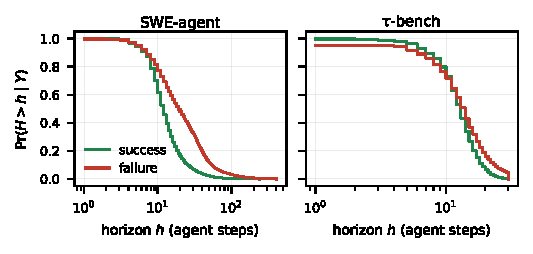
\includegraphics[width=\columnwidth]{figures/fig2_horizon_survival.pdf}
\caption{Horizon survival $\Pr(H>h\mid Y)$ for successful and failed runs
(log scale).\rev{} SWE-agent successes are much shorter; on $\tau$-bench the
curves nearly coincide and cross at short horizons, so first-order stochastic
dominance fails in both corpora.}
\label{fig:horizon}
\end{figure}

\paragraph{A.4 Monte Carlo.} For the predeclared analysis, 200 replicates per
hazard with $C_i\sim\mathrm{Bern}(\pi_i)$. Horvitz--Thompson bias never exceeds
$0.005$ points (SWE-agent) or $0.017$ ($\tau$-bench); its standard deviation
grows from $0.018$ to $0.097$ points (SWE-agent) and $0.13$ to $0.60$
($\tau$-bench) as $q$ goes from $0.1\%$ to $2\%$. Realised complete-case means
agree with the induced estimand within $0.001$ points (SWE-agent) and $0.04$
($\tau$-bench, within Monte Carlo error). The revision analyses (A.6) simulate
failure times $T_i$ step by step, which the Kaplan--Meier estimator needs.

\paragraph{A.5 Task-balanced results.} Weighting each task equally: SWE-agent
$p=9.80\%$ with $q{=}1\%$ biases $+1.14/-1.30$ and $q{=}2\%$ biases
$+2.04/-2.36$; $\tau$-bench $p=56.93\%$ with $+0.22/-7.29$ and $+0.37/-13.61$.
Absolute reliability depends on the weighting; the direction of both
distortions does not.

\paragraph{A.6 Misspecified hazard and hard caps.} SWE-agent unless stated,
200 replicates.
\emph{Predeclared stress test:} hazard $q_0$ up to step 25 and $2q_0$ beyond,
weighted with known constant-hazard $\pi=(1-q_0)^H$: at $q_0=0.5\%$ HT bias
$-0.14$, H\'ajek $+0.55$ points; at $q_0=1\%$, $-0.26$ and $+0.97$.
\emph{Revision\rev, weights estimated from $(V_i,C_i)$:} Kaplan--Meier H\'ajek
$+0.003$ and $+0.024$; constant-$\hat q$ H\'ajek $+0.33$ and $+0.67$. On
$\tau$-bench the same comparison gives $+0.002$/$-0.004$ (KM) and
$+0.036$/$+0.066$ (constant $\hat q$).
\emph{Hard caps\rev} (every run longer than $K$ steps invalid, deterministic):
on SWE-agent, $K=25$ invalidates 34.7\% of runs, the complete-case and
Kaplan--Meier estimates are both 23.04\%, invalid-as-failure 15.05\%, and the
bounds $[15.05,49.73]\%$ (true 16.73\%); $K=50$ invalidates 9.9\% with
estimates 18.17\% and 16.36\% and bounds $[16.36,26.31]\%$. On $\tau$-bench
$K=25$ invalidates 4.1\% (estimates 56.71\% and 54.36\%, bounds
$[54.36,58.51]\%$, true 55.03\%).

\paragraph{A.7 Exit statuses and observed container failures.}
Table~\ref{tab:exit} applies Definition~1 to SWE-agent's exit statuses, whose
meanings we read from the SWE-agent source \citep{sweagent2024code}.

\begin{table}[h]
\centering
\footnotesize
\setlength{\tabcolsep}{1.8pt}
\begin{tabular}{@{}lrrl@{}}
\toprule
exit status & $n$ & res.\,\% & class \\
\midrule
\texttt{submitted} & 51{,}087 & 24.8 & outcome \\
\texttt{submitted (exit\_context)} & 21{,}026 & 3.4 & context \\
\texttt{exit\_context} & 3{,}568 & 0 & context \\
\texttt{early\_exit} & 3{,}176 & 0 & unattributable \\
\texttt{submitted\_no\_patch} & 1{,}066 & 0 & outcome \\
\texttt{submitted (exit\_format)} & 80 & 6.2 & format \\
\texttt{exit\_format} & 20 & 0 & format \\
\texttt{submitted (exit\_cost)} & 10 & 0 & budget \\
\texttt{exit\_cost} & 3 & 0 & budget \\
\bottomrule
\end{tabular}
\caption{SWE-agent exit statuses classified by Definition~1.\rev{} All
classes except \emph{unattributable} are valid outcomes: \emph{context} and
\emph{budget} are declared-resource exhaustion and \emph{format} is repeated
malformed agent output. \texttt{early\_exit} is a container runtime error that
may or may not follow an agent command.}
\label{tab:exit}
\end{table}

\noindent\texttt{early\_exit} counts by
model: 3{,}170 of 74{,}792 runs (llama-70b), 6 of 4{,}053 (llama-8b), 0 of
1{,}191 (llama-405b). Hazard per run-step by step band 1--10/11--25/26--50/
51--100/101+: 0.13/0.18/0.15/0.11/0.22\%. Unstratified Kaplan--Meier gives
17.10\%. A task-cluster bootstrap (200 resamples) gives $[15.7,18.3]\%$ for the
stratified estimate; this interval reflects sampling of tasks, a population
question the finite-corpus analysis otherwise avoids.

\paragraph{A.8 Reproduction.} Two commands regenerate every number and
Figure~\ref{fig:main} without any paid API: the predeclared results, then the
revision analyses.

\smallskip
{\small\raggedright
\texttt{uv run python scripts/censoring/reproduce\_all.py}\\
\texttt{uv run python scripts/censoring/revision\_analysis.py}\par}
\smallskip

\noindent Summaries, audits, and provenance (dataset revisions, retrieval
dates, licenses) are written to \texttt{results/censoring/}. $\tau$-bench
declares no license, so only derived statistics are stored.

\paragraph{A.9 Prior controlled measurement cases.} The artifact also
demonstrates four non-censoring invalidity sources: omitting the official
evaluator test patch (pytest exits 4, ``no tests ran''), pipeline exit-code
masking without \texttt{pipefail}, container-wide rather than repository-scoped
change attribution ($0\!\to\!32$ files from environment churn alone), and
future/oracle leakage (20 adversarial future steps alter 0 of 24 prefix
features).

\end{document}
